\section{Hydra}

\nocite{adams1995hitchhiker}

%% XXX: show the hydra protocol here..

There are at least two fundamental problems one must address in any access control
system: (1) how access control policies are represented and (2) how they are enforced.
Policy representation specifies how policies are mapped onto resources (or content).
For example, one representation might map content names to sets of public keys. These
keys could be owned by authorized consumers and are used when encrypting content.
Encrypting content with name $N$ under a key $pk$ restricts access to the owner of
the corresponding private key. The challenge is to devise a representation that
scales well with the number of resources (content) and consumers. Regardless of
the approach, we claim there is one fundamental feature that must be present for
every access control decision: consumer requests must be bound to a principal.
This allows the producer or entity serving data to provide the appropriate
representation of the target data to the consumer. To achieve this goal, Hydra
uses AccessIDs described in the previous section.

The second problem is rooted more in system design. Consider what must be done
to satisfy a request for access-controlled content. First, the requestor must
be authenticated to bind the request to a principal. Second, the request must
be authorized to determine if access to the desired content is permissable. Lastly,
the data must be packaged in a protected (encrypted) form for the requestor. Thus,
problem (2) is more about how entities are configured to handle the separate
authentication, authorization, content distribution steps in CCN.

In past work, these roles were often convoluted. In particular, \cite{pre,be}
assumed that the entity which handles data production was also implicitly
responsible for content authentication and authorization. CCN-AC \cite{xx} and
NDN-NBAC \cite{xx} separated the authentication and authorization service from
the data production. Specifically, data owners generate and distribute consumer (principal)
private keys to consumers through out-of-band channels. Data producers receive
the corresponding public keys through a similar channel. These are used to encrypt
randomly generated per-content encryption keys.

Despite this separation, these designs still suffer from the following problems.
{\bf First}, authentication and authorization are unnecessarily coupled, leading
to an inherent ``time of check'' versus ``time of use'' problem. Specifically,
consumers obtain private keys from the data owner at time $t$ and use them to
decrypt content at time $t' > t$. {\bf Second}, if consumers are forced to fetch
their private keys from the data owner, a single point of failure emerges. In
particular, it becomes easy to launch a Denial of Service (DoS) attack on the
data owner by forcing it to perform expensive cryptographic operations, e.g.,
signature verifications.
%% @Ivan, the reasons above are ridiculous -- please add others!

Hydra is a system designed to address these problems. It has the following features:
%
\begin{compactitem}
    \item Consumer authentication and content authorization decisions can be separated
    and performed by separate systems in the network. A Hydra administrator can spawn
    any number of authentication endpoints to handle client authentication requests.
    Consumers are unable to fetch data from the authorization agent without having
    first been authenticated.
    \item Authorization decisions are centralized to a single system (or set of synchronized
    systems). This permits each authorization check to be done in real-time without
    introducing any added delay between the subsequent use.
    \item XXX
    \item XXX
    \item XXX
\end{compactitem}
%

\begin{table}
\centering
\caption{Notation summary}
\label{notation}
\begin{tabular}{|l|p{6cm}|}
\hline
Notation    			&  Description  							\\ \hline \hline
$I.name$			&  Name of the issued interest I					\\&\\
$N$				&  A namespace prefix (e.g., /uci/ics/ivan/\*) 				\\&\\
$TGT\_Name$			&  Ticket-granting-ticket name (e.g., /uci/ics/TGT) that will be routed towards authenticator \\&\\
$TGS\_Name$			&  Ticket-granting-service name (e.g., /uci/ics/TGS) that will be routed towards authorizer   \\&\\
$sk_C$      			&  Consumer Secret Key						        \\&\\
$pk_C$			        &  Consumer Public Key, including public UID and certificate        	\\&\\
$k_A$ 	   		 	&  Long term symmetric key shared between Authenticator and Authorizer  \\&\\
$k_P$ 	   		 	&  Long term symmetric key shared between Authenticator and Producer    \\&\\
$s \sample \{0,1\}^{\lambda}$	&  Random ${\lambda}$-bits number generation    	     		\\&\\
$ct = Enc_{k}(pt) $		&  Authenticated Encryption of $pt$ using symmetric key $k$		\\&\\
$pt = Dec_{k}(ct) $		&  Decryption of $ct$ using symmetric key $k$    	     		\\&\\
$ct = Enc_{pk}(pt) $		&  Authenticated Encryption of $pt$ using public key $pk$ 		\\&\\
$pt = Dec_{sk}(ct) $		&  Decryption of $ct$ using secret key $sk$    	     			\\&\\
$\sigma = Sign_{sk}(m) $	&  Signature on message $m$ using secret key $sk$ 			\\&\\
$Verif_{pk}(\sigma,m) $		&  Signature verification using public key $pk$     			\\&\\
\hline
\end{tabular}
\end{table}

\begin{figure}
\begin{center}
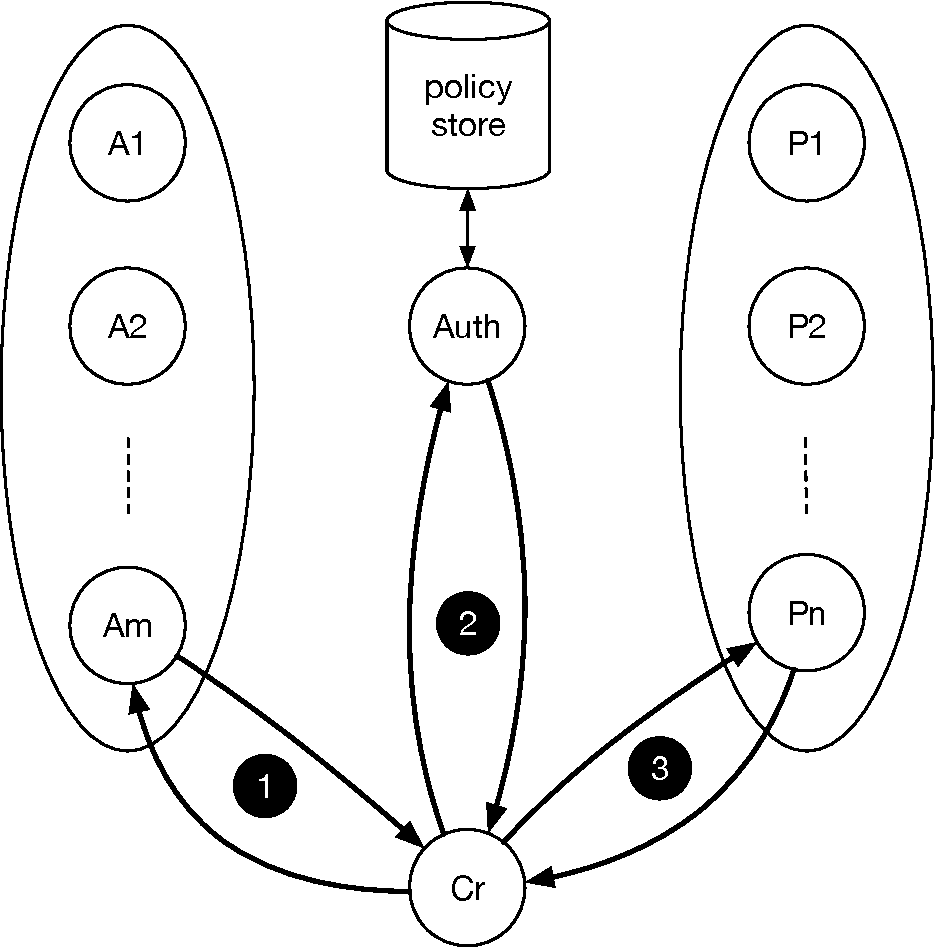
\includegraphics[width=\columnwidth]{Figures/hydra.pdf}
\caption{Hydra system design}
\label{fig:spectr-basic}
\end{center}
\end{figure}




\begin{figure*}
\begin{center}
\fbox{
\procedure{}{%
\textbf{Consumer} \> \> \textbf{Authenticator} \\
\mathsf{I.name = TGT\_Name} \> \> \\
\sigma \gets \mathsf{Sign}_{sk_C}(\mathsf{userName}) \> \> \\
\> \xrightarrow{payload = \sigma, userName} \> \\
\> \> \text{Fetch $pk_C$ according to userName} \\
\> \> \mathsf{Verify}_{pk_C}(\sigma,\mathsf{userName}) \\
%\> \> s \sample \{0,1\}^{\lambda} \\
\> \> t_1 \gets \mathsf{setTGTExpiration}() \\
\> \> k_{TGS} \sample \{0,1\}^{\lambda} \\
\> \> \mathsf{token}_{TGS}^{C} \gets \mathsf{Enc}_{pk_C}(k_{TGS}||t_1) \\
\> \> \mathsf{TGT} \gets \mathsf{Enc}_{k_{A}}(\mathsf{userName} || t_1 || k_{TGS}) \\
\> \xleftarrow{payload = \mathsf{TGT}, \mathsf{token}_{TGS}^{C}} \> \\
k_{TGS}||t_1 \gets \mathsf{Dec}_{sk_C}(\mathsf{token}_{TGS}^{C}) \> \> \\
\mathsf{store(TGT,t_1,k_{TGS})} \> \> \\
}
}
\caption{Consumer authentication protocol}
\label{fig:spectr-basic}
\end{center}
\end{figure*}




\begin{figure*}
\begin{center}
\fbox{
\procedure{}{%
\textbf{Consumer} \> \> \textbf{Authorizer} \\
\mathsf{I.name = TGS\_Name} \> \> \\
\> \xrightarrow{payload=N, \mathsf{TGT}} \> \\
\> \> \mathsf{userName} || t_1 || k_{TGS} \gets \mathsf{Dec}_{k_{A}}(TGT) \\
%\> \> \text{Verify: $s = s'$} \\
\> \> \text{Verify: $t_1$ not expired} \\
\> \> {k_P} \gets \mathsf{verifyPolicyAndFetchKey}(N, \mathsf{userName}) \\ %Kp can be different things (shared key between all boxes that implement that producer, broadcast encryption key, etc)
\> \> k_{N} \sample \{0,1\}^{\lambda} \\
%\> \> r \sample \{0,1\}^{\lambda} \\ why?
\> \> t_2 \gets \mathsf{setTGSExpiration}() \\ %% timestamp
\> \> \mathsf{TGS} \gets \mathsf{Enc}_{k_P}( N || k_N || t_2) \\ %% encrypt the key in the ticket
\> \> \mathsf{token}_N^{C} \gets \mathsf{Enc}_{k_{TGS}}(k_N||t_2) \\
\> \xleftarrow{payload= \mathsf{TGS}, \mathsf{token}_N^{C}} \> \\
k_N || t_2 \gets \mathsf{Dec}_{k_{TGS}}(\mathsf{token}_N^{C}) \> \\
\mathsf{store(N,TGS,t_2,k_N)} \>
}
}
\caption{Consumer-data authorization protocol}
\label{fig:spectr-basic}
\end{center}
\end{figure*}

\begin{figure*}
\begin{center}
\fbox{
\procedure{}{%
\textbf{Consumer} \> \> \textbf{Producer} \\
\mathsf{I.name = N||suffix} \> \> \\
\> \xrightarrow{payload= TGS} \> \\
\> \>  N' || k_N || t_2 \gets \mathsf{Dec}_{k_P}(TGS) \\
\> \> \text{Verify: $N'$ is prefix of I.name} \\
%%\> \> \text{Verify: $pk_C'$ = $pk_C$} \\ Not sure this is necessary
\> \> \text{Verify $t_2$ expiration} \\
\> \> D \gets \mathsf{ProduceData}(\mathsf{I.name}) \\
\> \> D' \gets \mathsf{Enc}_{k_N}(D) \\
\> \xleftarrow{payload=D'} \> \\
D \gets \mathsf{Dec}_{K_N}(\mathsf{D'}) \> \> \\
}
}
\caption{Consumer-data authorization protocol}
\label{fig:spectr-basic}
\end{center}
\end{figure*}

\subsection{Ivan: Comments}
\begin{enumerate}
 \item IMO, the authentication algorithm (Fig.2) should be unrelated to the namespace you want to get access to. Only related to Consumer's claimed Identity. Otherwise the consumer has to go back to the Authenticator every time she wants a different content (3 RTT).
 \item Unless we are assuming that there is some magical non-deterministic router that will route the same name through different paths, I.name must specify the content produced by the Authenticator, i.e., the TGT. The same applies for TGS.
 \item The TGT as a MAC never expires. My suggestion is to encrypt a timestamp, as in Kerberos, and as we are doing in the authorizer. MAC with an epoch is also an option, but not a good one.
 \item PKE of $K_N$ in the authorization algorithm (Fig 3) could (and maybe should) be symmetric AEAD.
 \item $verifyPolicyAndFetchKey()$ : Could be implemented as broadcast encryption...
 \item Consumer has to receive the expiration date of TGT/TGS. This way Consumer can get back to Authenticator/Authorizer directly, without issuing expired TGT/TGS messages to authorizer/producers.
\end{enumerate}